\section{多元向量值函数的微分}
\label{sec:multivariable-vector-differentiation}

前面每个输入只产生一个实数。本节研究同时产生$m$个输出分量的映射$F:U\subseteq\mathbb R^d\to\mathbb R^m$，关心输入稍作改变时输出点整体怎样移动。

例如极坐标映射$(r,\theta)\mapsto(r\cos\theta,r\sin\theta)$把两个参数变成平面上的点，神经网络的一层把输入向量变成另一个向量；参数曲线（$d=1$）与参数曲面（$d=2$、$m=3$）也是这种映射。
输出只有有限个分量，所以可以逐个分量使用前面的结论。但每个分量仍要对全部输入方向整体扰动，不能用坐标切片代替各分量的全微分。本节先用一个线性映射定义整体可微并引入Jacobian矩阵，再给出复合映射的导数，最后用导数的算子范数估计有限增量。

\subsection{Jacobian矩阵}

向量值函数由它的全部输出分量确定，因此按分量书写。
\begin{definition}[多元向量值函数]
\label{def:multivariable-vector-function}
映射$F:U\subseteq\mathbb R^d\to\mathbb R^m$称为多元向量值函数，写作$F=(F_1,\ldots,F_m)^\top$，其中每个$F_i:U\to\mathbb R$为多元标量函数。
\end{definition}
向量值函数的极限与连续性已在第~\ref{sec:multivariable-joint-limit-section}节与第~\ref{sec:multivariable-continuity}节定义，第~\ref{sec:multivariable-field-limits-continuity}节回顾了要点：输出点整体接近，等价于每个输出分量接近；每个分量的极限仍是对全部输入方向的联合极限。本节在连续性的基础上进一步研究线性近似。向量场是$m=d$的特例，下面的结论对它同样适用。

\paragraph{微分与Jacobian矩阵}

标量输出的全微分是到实数的线性映射，也称线性泛函。向量输出的全微分则要把输入扰动映射为$m$维输出扰动。
有限维线性映射由矩阵表示，矩阵的每一行记录一个输出分量的系数。
\begin{definition}[向量值函数的微分]
\label{def:multivariable-vector-differential}
设$U$开，$F:U\to\mathbb R^m$，$\bm a\in U$。若存在线性映射$\mathrm dF_{\bm a}:\mathbb R^d\to\mathbb R^m$，记它在标准基下的矩阵为$\bm J_F(\bm a)\in\mathbb R^{m\times d}$，使
\begin{equation}
 F(\bm a+\bm h)=F(\bm a)+\bm J_F(\bm a)\bm h+o(\lVert\bm h\rVert_2),
\label{eq:analysis-jacobian-linearization}
\end{equation}
则称$F$在$\bm a$处可微，余项按输出欧氏范数理解。
$\mathrm dF_{\bm a}(\bm h)=\bm J_F(\bm a)\bm h$称为$F$在$\bm a$处的微分，矩阵$\bm J_F(\bm a)$称为\term{Jacobian矩阵}（Jacobian matrix）。
\end{definition}
向量值函数可微当且仅当每个输出分量$F_i$可微。正向只需从向量余项取第$i$个分量，它的绝对值不超过向量余项的欧氏长度，于是得到$F_i$的标量展开；反向则把有限个分量的$o(\lVert\bm h\rVert_2)$余项用欧氏范数合并，合并后仍是$o(\lVert\bm h\rVert_2)$。
由此，Jacobian的第$i$行是分量梯度的转置$\nabla F_i^\top$，第$i,j$个元素为$\partial_jF_i$；微分若存在则唯一。$C^k$向量值函数指所有输出分量都属于$C^k$。

本书把输入、输出都写成列向量，因此$\bm J_F(\bm a)$是“输出维数$\times$输入维数”的矩阵：第$i$行记录第$i$个输出对各输入的偏导数，$\bm J_F(\bm a)\bm h$的形状为$(m\times d)(d\times1)=m\times1$，与输出一致。$m=1$时Jacobian是$1\times d$的行向量$\nabla f(\bm a)^\top$，梯度则是列向量，二者互为转置。

\paragraph{Jacobian矩阵的几何意义}
按行看，Jacobian记录各输出分量的梯度；按列看，它记录各输入坐标对输出点的推动。第$j$列
\[
 \bm J_F(\bm a)\bm e_j=(\partial_jF_1,\ldots,\partial_jF_m)^\top
\]
表示：只把第$j$个输入增加一个很小的量$t$时，输出点大约移动这个向量的$t$倍。一般扰动$\bm h=\sum_jh_j\bm e_j$的一阶效果，就是这些列按$h_j$加权求和。
对$d=m=2$，由此得到局部伸缩的图像。以$\bm a$为角、边长为$\varepsilon$的小正方形由$\varepsilon\bm e_1,\varepsilon\bm e_2$张成，它的像近似是由$\varepsilon\bm J_F\bm e_1,\varepsilon\bm J_F\bm e_2$张成的平行四边形。行列式的绝对值是线性映射对面积的缩放倍数（第~\ref{sec:prelim-determinants}节），所以像的面积约为$|\det\bm J_F(\bm a)|\varepsilon^2$；行列式的符号说明局部是否翻转了定向。

极坐标映射是这种局部伸缩的一个具体例子。
\begin{example}[极坐标映射的Jacobian矩阵]
\label{ex:multivariable-polar-jacobian}
考虑极坐标映射
\[
 P(r,\theta)=(r\cos\theta,r\sin\theta)^\top.
\]
逐个输出分量求偏导，得到
\[
\begin{gathered}
\bm J_P(r,\theta)=\begin{bmatrix}\cos\theta&-r\sin\theta\\ \sin\theta&r\cos\theta\end{bmatrix}\\
\det\bm J_P=r\cos^2\theta+r\sin^2\theta=r.
\end{gathered}
\]
第一列是单位径向向量：$r$增加$\mathrm dr$，点沿射线向外移动$\mathrm dr$。第二列长度为$r$、沿圆周切向：$\theta$增加$\mathrm d\theta$，点沿半径为$r$的圆移动约$r\,\mathrm d\theta$。因此参数平面中面积为$\mathrm dr\,\mathrm d\theta$的小矩形，变成面积约为$r\,\mathrm dr\,\mathrm d\theta$的小扇形块。
\end{example}

离原点越远，同样的角度增量扫过的弧越长，面积放大越多。第~\ref{sec:classical-change-variables}节的区域积分换元就用这个倍数校正面积。

对一般的非线性映射，小网格块的像是弯边块，线性近似把它换成平行四边形。图~\ref{fig:analysis-process-jacobian-grid-cell}画出了这种对应。图中$\det J_T(a)=1\times0.6-0.25\times0.3=0.525$，所以绿色小方块的像面积约为原面积的一半。
\begin{figure*}[!htbp]
 \centering
 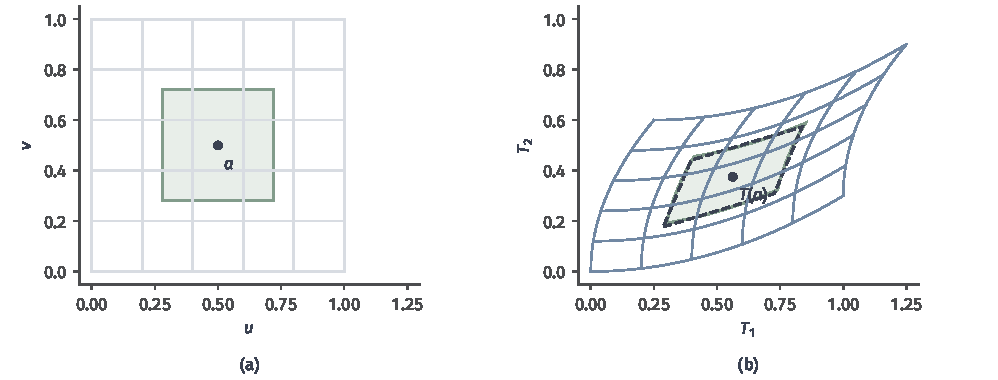
\includegraphics[width=169.0mm]{figures/00-shared/mathematical-preliminaries-upper/00-shared/matplotlib/chapter3-concept-processes/jacobian-grid-cell.pdf}
 \caption{取$T(u,v)=(u+v^2/4,\,0.6v+0.3u^2)$，$a=(0.5,0.5)$。(a) 输入网格及绿色小方块。(b) 非线性像为弯边块，黑虚线为$T(a)+J_T(a)(h,k)^\top$给出的平行四边形；$J_T(a)=\bigl[\begin{smallmatrix}1&0.25\\0.3&0.6\end{smallmatrix}\bigr]$。有限块不与线性像完全重合，缩小扰动后才由可微余项控制差异。}
 \label{fig:analysis-process-jacobian-grid-cell}
\end{figure*}

输入、输出维数不同时，同一个原则给出非方阵的Jacobian。
\begin{example}[空间螺旋线的Jacobian矩阵]
\label{ex:multivariable-helix-jacobian}
令$\bm\gamma(t)=(\cos t,\sin t,t)^\top$，$t\in\mathbb R$，输入一维、输出三维。逐分量求导得
\[
 \bm J_{\bm\gamma}(t)=\begin{bmatrix}-\sin t\\ \cos t\\ 1\end{bmatrix}\in\mathbb R^{3\times1}.
\]
它把参数增量$s$映为$s\bm J_{\bm\gamma}(t)$：点沿速度向量$\bm\gamma'(t)$移动。这一列就是曲线的切向量，长度为$\sqrt2$，说明参数每增加一个单位，点约移动$\sqrt2$的距离。
\end{example}
螺旋线的Jacobian不是方阵，没有行列式可言，局部伸缩由切向量的长度描述。极坐标与螺旋线说明，“微分是线性映射”这一原则在不同输入、输出维数下给出形状不同的矩阵，不能默认Jacobian是方阵或有行列式。梯度映射$\bm x\mapsto\nabla f(\bm x)$本身也是从$\mathbb R^d$到$\mathbb R^d$的向量值映射，第~\ref{sec:multivariable-curvature-error}节将研究它的微分，并由此得到Hessian矩阵。

\paragraph{Jacobian矩阵的计算}
计算Jacobian矩阵时，先把每个输出分量当作标量函数求偏导，再按行排列；排好后核对矩阵形状是否为“输出维数$\times$输入维数”。
例如$F(x,y)=(x^2+xy,y^2)^\top$的Jacobian为
\[
 \bm J_F(x,y)=\begin{bmatrix}2x+y&x\\0&2y\end{bmatrix}.
\]
在$(1,2)$处，它把扰动$(h,k)^\top$的一阶影响写成$(4h+k,4k)^\top$。第一行说明第一个输出同时受两个输入推动，第二行说明第二个输出只随$y$变化；两列分别记录沿$x$、沿$y$移动时输出点的位移方向。

再看机器学习中常用的一个向量值映射。它把任意一组实数变成总和为$1$的正权重：先取指数，再除以共同的总和。
这就是$n$维\term{归一化指数映射}（softmax），分类模型常用它把各类别的得分变成概率。对正整数$n$和
$\bm{z}\in\mathbb{R}^n$，令
\[
 \begin{gathered}
s_i(\bm{z})
  =
  \frac{e^{z_i}}{\sum_{k=1}^n e^{z_k}}\\
i=1,\ldots,n.
 \end{gathered}
\]
记分母为$Z=\sum_k e^{z_k}$，它对$z_j$的偏导数为$e^{z_j}$。对分子$e^{z_i}$求偏导，$i=j$时得$e^{z_i}$，$i\neq j$时得$0$，记为$\mathbb{I}\{i=j\}e^{z_i}$。商法则给出
\[
  \frac{\partial s_i}{\partial z_j}
  =
  \frac{\mathbb{I}\{i=j\}e^{z_i}Z-e^{z_i}e^{z_j}}{Z^2}
  =
  s_i\bigl(\mathbb{I}\{i=j\}-s_j\bigr).
\]
因此整个Jacobian矩阵为
\begin{equation}
  \bm{J}_{\bm{s}}(\bm{z})
  =
  \operatorname{diag}(\bm{s})-\bm{s}\bm{s}^{\top}.
\label{eq:analysis-softmax-jacobian}
\end{equation}
这里$\operatorname{diag}(\bm s)$表示以$s_1,\ldots,s_n$为对角元、其他元素为零的对角矩阵。

当$n\geq2$时，对角项$s_i(1-s_i)$为正，描述提高$z_i$对自身分量的影响。非对角项$-s_is_j$为负，它来自共同分母：提高一个得分会压低其余分量。当$n=1$时输出恒为$1$，Jacobian为零。

每行元素之和为$s_i-s_i\sum_js_j=0$。这与给所有$z_i$加同一常数不改变输出相符：沿方向$(1,\ldots,1)^\top$的一阶变化为零。

在最简单的情形中，可以用数值核对式~\eqref{eq:analysis-softmax-jacobian}给出的线性近似。
\begin{example}[二维softmax的Jacobian矩阵]
\label{ex:multivariable-softmax-jacobian-check}
取$n=2$、$\bm z=\bm 0$，则$\bm s=(1/2,1/2)^\top$，由式~\eqref{eq:analysis-softmax-jacobian}，
\[
 \bm J_{\bm s}(\bm 0)
 =\begin{bmatrix}1/2&0\\0&1/2\end{bmatrix}-\begin{bmatrix}1/4&1/4\\1/4&1/4\end{bmatrix}
 =\begin{bmatrix}1/4&-1/4\\-1/4&1/4\end{bmatrix}.
\]
把$z_1$提高$0.1$，线性近似给出$\bm s$的增量约为
\[
 \bm J_{\bm s}(\bm 0)(0.1,0)^\top=(0.025,-0.025)^\top,
\]
即$s_1\approx0.525$、$s_2\approx0.475$。实际值为$s_1=e^{0.1}/(e^{0.1}+1)\approx0.52498$、$s_2\approx0.47502$。
\end{example}

线性近似与实际值只差约$2\times10^{-5}$，远小于输入改变量$0.1$；两个分量的增量一正一负、总和为零，与$s_1+s_2$恒为$1$相符。

\subsection{微分的运算法则}
\label{sec:analysis-vector-chain-matrix-calculus}

与标量情形一样，复杂映射的Jacobian可以由简单映射的Jacobian组合得到。各法则以运算有定义为前提：输出形状相同的向量值函数可以相加、相减，任何向量值函数都可以数乘；复合则要求前一映射的输出落在后一映射的定义域内。
两个向量之间的乘法需要先指定含义；下面先处理线性运算与复合，再用链式法则处理内积等乘法结构。

\paragraph{和、差与数乘的微分}
若$F,H:U\to\mathbb R^m$在$\bm a$处可微，对每个输出分量分别使用标量的和、差与数乘法则，再把各分量的结果按行排回矩阵，得到
\[
 \begin{gathered}
 \bm J_{F\pm H}(\bm a)=\bm J_F(\bm a)\pm\bm J_H(\bm a)\\
 \bm J_{cF}(\bm a)=c\bm J_F(\bm a),
 \end{gathered}
\]
其中$c$是固定实数。相加的输出形状以及两个Jacobian的形状必须分别一致。

\paragraph{复合函数的链式法则}
复合映射$G\circ F$先用$F$把输入变成中间量，再用$G$把中间量变成输出。输入的小扰动$\bm h$先被$F$变成中间量的扰动，一阶上约为$\bm J_F\bm h$；这个扰动再被$G$变成输出扰动，一阶上约为$\bm J_G(\bm J_F\bm h)$。
所以复合映射的Jacobian是两个Jacobian按计算顺序的乘积。与一元情形一样，这项规则称为\term{链式法则}（chain rule）。
\begin{theorem}[向量值函数的链式法则]
\label{thm:multivariable-vector-chain-rule}
设$U\subseteq\mathbb R^d$、$V\subseteq\mathbb R^m$开，$F:U\to V$在$\bm a$处可微，$G:V\to\mathbb R^p$在$F(\bm a)$处可微，则$G\circ F$在$\bm a$处可微，且
\begin{equation}
 \bm J_{G\circ F}(\bm a)=\bm J_G(F(\bm a))\bm J_F(\bm a).
\label{eq:analysis-vector-chain-rule}
\end{equation}
\end{theorem}
\begin{proof}
记$\bm A=\bm J_F(\bm a)$、$\bm B=\bm J_G(F(\bm a))$。由$F$可微，中间量的增量为
\[
 \bm k=F(\bm a+\bm h)-F(\bm a)=\bm A\bm h+o(\lVert\bm h\rVert_2),
\]
故$\lVert\bm k\rVert_2\leq\lVert\bm A\bm h\rVert_2+o(\lVert\bm h\rVert_2)=O(\lVert\bm h\rVert_2)$：中间量的扰动与原扰动同阶。
代入$G$的一阶展开，
\[
 G(F(\bm a)+\bm k)-G(F(\bm a))=\bm B\bm k+o(\lVert\bm k\rVert_2)
 =\bm B\bm A\bm h+\bm B\,o(\lVert\bm h\rVert_2)+o(\lVert\bm k\rVert_2).
\]
右侧第二项中，矩阵$\bm B$至多把长度放大固定倍数，所以仍是$o(\lVert\bm h\rVert_2)$；第三项因$\lVert\bm k\rVert_2=O(\lVert\bm h\rVert_2)$也是$o(\lVert\bm h\rVert_2)$（$\bm k=\bm0$时外层余项为零）。
于是复合增量等于$\bm B\bm A\bm h$加上$o(\lVert\bm h\rVert_2)$，这正是复合函数的可微定义。
\end{proof}
式~\eqref{eq:analysis-vector-chain-rule}中的矩阵形状为$(p\times m)(m\times d)=p\times d$，反向相乘往往没有定义。
即使两个次序都有定义，矩阵乘法一般也不交换，不能按标量经验调换因子。
用局部伸缩的语言说，复合映射在一点附近的伸缩等于两步伸缩依次作用。方阵情形下，由行列式的乘法公式，面积缩放倍数也相乘。

\paragraph{内积、范数平方与复合二次型}
链式法则把复杂表达式拆成一串简单映射；计算时要分清哪些对象是向量值中间变量，哪些是最后的标量。设$F,G:U\to\mathbb R^m$在$\bm a$处可微。内积$\phi(\bm x)=F(\bm x)^\top G(\bm x)$是映射$\bm x\mapsto(F(\bm x),G(\bm x))\in\mathbb R^{2m}$与双线性函数$b(\bm u,\bm w)=\bm u^\top\bm w$的复合。$b$在$(\bm u,\bm w)$处的精确增量为
\[
 b(\bm u+\bm p,\bm w+\bm r)-b(\bm u,\bm w)=\bm p^\top\bm w+\bm u^\top\bm r+\bm p^\top\bm r,
\]
末项满足$|\bm p^\top\bm r|\leq\lVert\bm p\rVert_2\lVert\bm r\rVert_2\leq\tfrac12(\lVert\bm p\rVert_2^2+\lVert\bm r\rVert_2^2)$，是联合扰动的二次量，所以$b$可微，微分为$(\bm p,\bm r)\mapsto\bm p^\top\bm w+\bm u^\top\bm r$。由链式法则，
\[
 \begin{gathered}
 \mathrm d\phi_{\bm a}(\bm h)=\bigl(\bm J_F(\bm a)\bm h\bigr)^\top G(\bm a)+F(\bm a)^\top\bm J_G(\bm a)\bm h\\
 \nabla\phi(\bm a)=\bm J_F(\bm a)^\top G(\bm a)+\bm J_G(\bm a)^\top F(\bm a).
 \end{gathered}
\]
取$G=F$，得到范数平方的梯度$\nabla\lVert F\rVert_2^2=2\bm J_F^\top F$。对固定的对称矩阵$\bm S$，复合二次型$F(\bm x)^\top\bm SF(\bm x)$是$F$与二次型$\bm y\mapsto\bm y^\top\bm S\bm y$的复合，由式~\eqref{eq:analysis-quadratic-form-gradient}和链式法则，梯度为$2\bm J_F^\top\bm SF$。

范数本身要单独判断。在$\bm x\neq\bm0$处，$\lVert\bm x\rVert_2=\sqrt{\lVert\bm x\rVert_2^2}$是正数上可微的平方根与光滑函数的复合，梯度为$\bm x/\lVert\bm x\rVert_2$。在原点，沿直线$t\bm v$（$\bm v\neq\bm0$）得到$|t|\lVert\bm v\rVert_2$，双侧方向导数不存在，所以不可微。范数平方在原点光滑，并不能推出范数在原点可微：平方根在$0$处没有有限导数，链式法则的条件不满足。

链式法则的一个常见用法是：先用向量值映射得到中间量，再把中间量变成一个标量，然后求这个标量对原输入的梯度。
\begin{example}[从中间向量求回复合目标的梯度]
\label{ex:analysis-chain-rule-calculation}
令
\[
 \begin{gathered}
F(x_1,x_2)=(x_1^2,x_1x_2,x_2)^\top\\
\ell(\bm y)=\frac12(y_1^2+y_2^2+y_3^2).
 \end{gathered}
\]
$F$从二维输入产生三维中间量，$\ell$再把三维中间量变成一个数，复合得到$L=\ell\circ F:\mathbb R^2\to\mathbb R$。
$\ell$的Jacobian是$1\times3$行向量$\nabla\ell(\bm y)^\top$，由链式法则，$L$的Jacobian为$\nabla\ell(F(\bm x))^\top\bm J_F(\bm x)$；转置后得到列向量梯度
\[
  \nabla L(\bm x)=\bm J_F(\bm x)^\top\nabla\ell\bigl(F(\bm x)\bigr).
\]
这里出现转置，是因为梯度按列向量书写，而链式法则中的$\ell$导数是行向量。本例中
\[
\begin{gathered}
\bm J_F=\begin{bmatrix}2x_1&0\\x_2&x_1\\0&1\end{bmatrix}\\
\nabla\ell(\bm y)=\bm y.
\end{gathered}
\]
在$\bm x=(1,2)^\top$处，$\bm y=(1,2,2)^\top$，链式法则给出
\[
  \nabla L(1,2)
  =\begin{bmatrix}2&2&0\\0&1&1\end{bmatrix}
    \begin{bmatrix}1\\2\\2\end{bmatrix}
  =\begin{bmatrix}6\\4\end{bmatrix}.
\]
也可以把复合函数直接展开为
$L(x_1,x_2)=\tfrac12(x_1^4+x_1^2x_2^2+x_2^2)$，求偏导得到
$\nabla L=(2x_1^3+x_1x_2^2,\,x_1^2x_2+x_2)^\top$，在同一点仍为$(6,4)^\top$。
矩阵形状$(2\times3)(3\times1)=2\times1$也核对了梯度传递的次序。
\end{example}

两种计算得到同一个梯度。链式形式保留了中间映射，各层的导数可以分别计算、分别复用。

\paragraph{梯度沿复合的传递与伴随}
例子中的转置不只是书写约定，它是第~\ref{sec:ls-adjoints}节的伴随。设$F:U\subseteq\mathbb R^d\to\mathbb R^m$在$\bm a$处可微，$g$在$F(\bm a)$的邻域内有定义并在$F(\bm a)$处可微，输入、输出空间各取一个内积。链式法则写成线性映射的复合$\mathrm d(g\circ F)_{\bm a}=\mathrm dg_{F(\bm a)}\circ\mathrm dF_{\bm a}$。对任意$\bm h$，依次使用梯度的定义与伴随的定义式~\eqref{eq:ls-adjoint-pairing}，
\[
 \mathrm d(g\circ F)_{\bm a}(\bm h)
 =\bigl\langle\nabla g(F(\bm a)),\mathrm dF_{\bm a}(\bm h)\bigr\rangle
 =\bigl\langle\mathrm dF_{\bm a}^\star\nabla g(F(\bm a)),\bm h\bigr\rangle,
\]
其中第一个内积在输出空间中计算，第二个在输入空间中计算。由梯度的唯一性，
\begin{equation}
 \nabla(g\circ F)(\bm a)=\mathrm dF_{\bm a}^\star\,\nabla g(F(\bm a)).
\label{eq:multivariable-gradient-adjoint}
\end{equation}
微分$\mathrm dF_{\bm a}$把输入扰动向前推到输出端，伴随则把输出端的梯度拉回输入端。两端都取标准欧氏内积时，伴随的矩阵是$\bm J_F(\bm a)^\top$，式~\eqref{eq:multivariable-gradient-adjoint}就是上例中的$\bm J_F^\top\nabla\ell$；两端分别取Gram矩阵为$\bm M_V,\bm M_W$的内积时，由式~\eqref{eq:ls-weighted-adjoint}，伴随的矩阵为$\bm M_V^{-1}\bm J_F(\bm a)^\top\bm M_W$，与式~\eqref{eq:multivariable-gradient-gram}相容。这样，矩阵乘法、泛函配对与梯度的传递是同一件事的三种写法；矩阵函数的梯度和隐函数的导数都沿用这一规则。

\subsection{向量增量的估计}
\label{sec:multivariable-vector-increment-bound}

标量函数的中值公式在线段上找到一个点，用那里的梯度精确表示增量。向量值函数不能照搬：各输出分量的一元中值点可能不同，没有一个共同的点代表整个向量增量。
例如$F(t)=(\cos t,\sin t)^\top$在$[0,2\pi]$上走完一整圈，$F(2\pi)-F(0)=\bm 0$，但速度$F'(t)=(-\sin t,\cos t)^\top$长度恒为$1$，不存在$\tau$使$F(2\pi)-F(0)=2\pi F'(\tau)$。
因此改为估计增量的长度，或者把增量写成沿线段的积分。

\paragraph{导数的算子范数}
\phantomsection
\label{def:analysis-induced-operator-norm}
对标量函数，导数的绝对值说明输入的小变化被放大多少倍。对向量输出，同一个线性映射在不同方向上的放大倍数可能不同，于是取其中最大的一个。第~\ref{sec:multivariable-operator-norm}节已经定义线性映射的算子范数，并证明有限维时它有限且可以取到。用于微分时，它度量最坏输入方向上的一阶放大倍数：
\[
 \lVert\mathrm dF_{\bm a}\rVert=\max_{\lVert\bm h\rVert\leq1}\lVert\mathrm dF_{\bm a}(\bm h)\rVert .
\]
两端都取欧氏范数时，它就是Jacobian矩阵的谱范数$\lVert\bm J_F(\bm a)\rVert_2$，并满足$\lVert\bm J_F(\bm a)\bm h\rVert_2\leq\lVert\bm J_F(\bm a)\rVert_2\lVert\bm h\rVert_2$。标量函数时$\lVert\nabla f(\bm a)^\top\rVert_2=\lVert\nabla f(\bm a)\rVert_2$，这就是上一节中梯度长度的角色。
计算时先给出对全部单位向量成立的上界，再找出达到上界的方向。
\begin{example}[对角矩阵的算子范数]
\label{ex:multivariable-diagonal-operator-norm}
令$\bm A=\operatorname{diag}(2,1)$，它把第一坐标放大两倍、第二坐标保持不变。对单位向量$\bm h$，
\[
 \lVert\bm A\bm h\rVert_2^2=4h_1^2+h_2^2\leq4(h_1^2+h_2^2)=4,
\]
且$\bm h=\bm e_1$时取等号，故$\lVert\bm A\rVert_2=2$。
\end{example}

又如旋转矩阵不改变任何向量的长度，算子范数为$1$。

用算子范数估计增量长度，就不再需要各分量共用一个中值点。所需条件是$G$在含整条线段的开集上连续可微。
\begin{theorem}[向量值函数的中值估计]
\label{thm:multivariable-vector-mean-value}
设$U\subseteq\mathbb R^r$开，$G:U\to\mathbb R^s$连续可微，且$[\bm y',\bm y]\subset U$，则
\begin{equation}
  \begin{aligned}
  \lVert G(\bm{y})-G(\bm{y}')\rVert_2
  &\leq
  \sup_{0\leq t\leq1}
  \left\lVert
    \bm J_G\bigl(\bm{y}'+t(\bm{y}-\bm{y}')\bigr)
  \right\rVert_2
  \lVert\bm{y}-\bm{y}'\rVert_2.
  \end{aligned}
\label{eq:analysis-operator-mean-value-bound}
\end{equation}
\end{theorem}
\begin{proof}
思路是把向量增量投影到它自己的方向上，变成一个标量函数的增量，再对标量函数用中值定理。若$\bm u=G(\bm y)-G(\bm y')\neq\bm0$，
取单位向量$\bm v=\bm u/\lVert\bm u\rVert_2$，并沿线段定义标量函数
$\phi(t)=\bm v^\top G(\bm y'+t(\bm y-\bm y'))$。
由链式法则，$\phi'(t)=\bm v^\top\bm J_G(\bm y'+t(\bm y-\bm y'))(\bm y-\bm y')$；中值定理给出某个$\tau\in(0,1)$，使
\[
 \lVert\bm u\rVert_2
 =\bm v^\top\bm u
 =\phi(1)-\phi(0)
 =\bm v^\top\bm J_G(\bm y'+\tau(\bm y-\bm y'))(\bm y-\bm y').
\]
对右侧先用内积不等式并注意$\lVert\bm v\rVert_2=1$，再用谱范数的上界，便得到式~\eqref{eq:analysis-operator-mean-value-bound}；
$\bm u=\bm0$时该界直接成立。
\end{proof}

\paragraph{向量增量的积分表示}
中值估计只给出长度的上界。在同样的条件下，还可以把整个向量增量精确写出。记$\bm p=\bm y-\bm y'$。对每个分量$G_i$，一元函数$t\mapsto G_i(\bm y'+t\bm p)$在$[0,1]$上连续可微，由式~\eqref{eq:multivariable-curve-chain-rule}，导数为$\nabla G_i(\bm y'+t\bm p)^\top\bm p$。逐分量使用一元微积分基本定理，得到
\begin{equation}
 G(\bm y)-G(\bm y')=\int_0^1\bm J_G(\bm y'+t\bm p)\,\bm p\,\mathrm dt,
\label{eq:multivariable-vector-integral-increment}
\end{equation}
其中向量的积分按分量理解。这个等式不需要共同的中间点：各分量的变化率沿整条线段累计。
对连续的向量值函数$\bm w:[0,1]\to\mathbb R^s$，有
\[
 \Bigl\lVert\int_0^1\bm w(t)\,\mathrm dt\Bigr\rVert_2\leq\int_0^1\lVert\bm w(t)\rVert_2\,\mathrm dt .
\]
记左侧的积分为$\bm u$，由积分的线性、单调性与Cauchy--Schwarz不等式，$\lVert\bm u\rVert_2^2=\int_0^1\bm u^\top\bm w(t)\,\mathrm dt\leq\lVert\bm u\rVert_2\int_0^1\lVert\bm w(t)\rVert_2\,\mathrm dt$，$\bm u\neq\bm0$时除以$\lVert\bm u\rVert_2$即得。把它用于式~\eqref{eq:multivariable-vector-integral-increment}，再次得到式~\eqref{eq:analysis-operator-mean-value-bound}。积分形式的长处在于，可以先从被积函数中扣除一个固定的线性项，第~\ref{chap:differential-perturbation-analysis}章据此估计一阶近似的余项（第~\ref{sec:multivariable-first-order-remainder}节）。

\paragraph{Lipschitz估计与压缩}
若定义域为凸开集，且Jacobian的谱范数在全域不超过同一个有限常数$L$，则由式~\eqref{eq:analysis-operator-mean-value-bound}，$G$以$L$为Lipschitz常数：任意两点的像之间的距离至多是原距离的$L$倍。在局部球上使用同样的界，就得到局部版本。
特别地，若Jacobian的谱范数在某个闭球内不超过常数$q<1$，映射就把球内任意两点间的距离缩小到至多$q$倍，称为压缩。但压缩界本身不保证迭代留在这个球内，也不单独给出不动点：还要检查映射把球映入自身，并借有限维空间的完备性（定理~\ref{thm:ls-finite-dimensional-complete}）取得迭代的极限。第~\ref{sec:analysis-implicit-parameter-integral}章证明隐函数定理时依次核对这三点。
